%!TEX TS-program = xelatex
\documentclass[]{friggeri-cv}
\usepackage{afterpage}
\usepackage{hyperref}
\usepackage{color}
\usepackage{xcolor}
\usepackage{smartdiagram}
\usepackage{fontspec}
% if you want to add fontawesome package
% you need to compile the tex file with LuaLaTeX
% References:
%   http://texdoc.net/texmf-dist/doc/latex/fontawesome/fontawesome.pdf
%   https://www.ctan.org/tex-archive/fonts/fontawesome?lang=en
%\usepackage{fontawesome}
\usepackage{metalogo}
\usepackage{dtklogos}
\usepackage[utf8]{inputenc}
\usepackage{tikz}
\usetikzlibrary{mindmap,shadows}
\hypersetup{
    pdftitle={},
    pdfauthor={},
    pdfsubject={},
    pdfkeywords={},
    colorlinks=false,           % no lik border color
    allbordercolors=white       % white border color for all
}
\smartdiagramset{
    bubble center node font = \footnotesize,
    bubble node font = \footnotesize,
    % specifies the minimum size of the bubble center node
    bubble center node size = 0.5cm,
    %  specifies the minimum size of the bubbles
    bubble node size = 0.5cm,
    % specifies which is the distance among the bubble center node and the other bubbles
    distance center/other bubbles = 0.3cm,
    % sets the distance from the text to the border of the bubble center node
    distance text center bubble = 0.5cm,
    % set center bubble color
    bubble center node color = pblue,
    % define the list of colors usable in the diagram
    set color list = {lightgray, materialcyan, orange, green, materialorange, materialteal, materialamber, materialindigo, materialgreen, materiallime},
    % sets the opacity at which the bubbles are shown
    bubble fill opacity = 0.6,
    % sets the opacity at which the bubble text is shown
    bubble text opacity = 0.5,
}

\addbibresource{bibliography.bib}
\RequirePackage{xcolor}
\definecolor{pblue}{HTML}{0395DE}

\begin{document}
  \vspace{1cm}
\header{Alcemir}{~R. Santos}
      {Software Engineer}
      
% Fake text to add separator      
\fcolorbox{white}{gray}{\parbox{\dimexpr\textwidth-2\fboxsep-2\fboxrule}{%
.....
}}

% In the aside, each new line forces a line break
\begin{aside}
  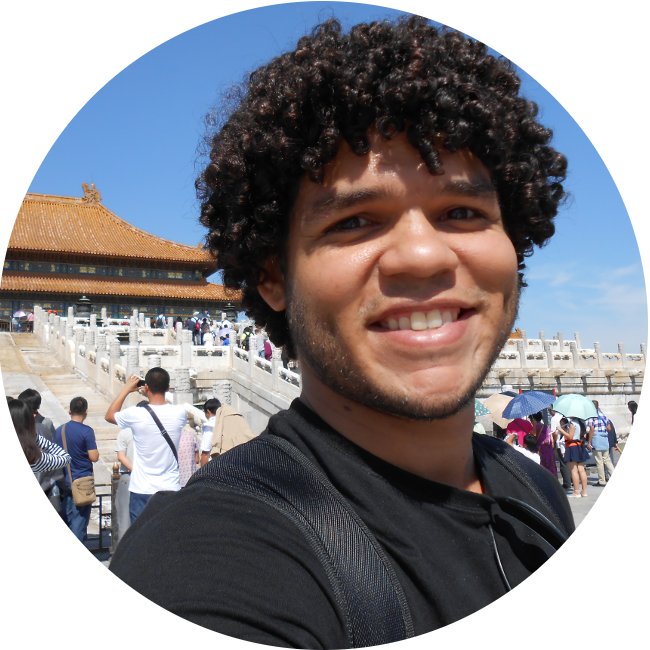
\includegraphics[scale=0.18]{img/eu-circle.png}
  \section{Address}
    Teresina
    Piauí, Brazil
    ~
  \section{Tel \& Skype}
    +55 71  99213 9611
    alcemir\_santos
    ~
  \section{Mail}
    \href{mailto:alcemir.santos@gmail.com}{\textbf{alcemir.santos@}\\gmail.com}
    ~
  \section{Web \& Git}
    \href{http://alcemirsantos.com}{alcemirsantos.com}
    \href{https://bitbucket.org/alcemirsantos}{alcemirsantos@bitbutcket}
        \href{https://github.com/alcemirsantos}{alcemirsantos@github}
    ~
  % use  \hspace{} or \vspace{} to change bubble size, if needed
  \section{Programming}
    \smartdiagram[bubble diagram]{
        \textbf{Java},
        \textbf{\vspace{2mm}Python\vspace{2mm}},
        \textbf{Objective C},
        \textbf{C/C++},
        \textbf{R},
        \textbf{PHP}
    }
    ~
  \section{Personal Skills}
    \smartdiagram[bubble diagram]{
        \textbf{Team}\\\textbf{Player},
        \textbf{Initiative},
        \textbf{Curiosity},
        \textbf{Problem}\\\textbf{Solving},
        \textbf{\vspace{2mm}Manage\vspace{2mm}},
        \textbf{Organize}
    }
    ~
\end{aside}
~
\section{Education}
\begin{entrylist}
     \entry
     {2014 - 2017?}
     {Ph.D in Computer Science}
     {Federal University of Bahia}
     {4 years scholarship grant from FAPESB.\\}
    \entry
    {2011 - 2013}
    {Master's Degree in Computer Science}
    {Federal University of Minas Gerais}
    {2 years scholarship grant from CNPq.\\}
    \entry
    {2006 - 2010}
    {Bachelor's Degree in Computer Science}
    {Federal University of Piauí}
    {2$^{nd}$ Best grade among the classmates.\\}
    \entry
    {2003 - 2005}
    {High School Diploma}
    {CEBRAPI}
    {3$^{rd}$ Best grade among the classmates.}
\end{entrylist}
\\
\section{Experience}
\begin{entrylist}
    \entry
    {2015 - 2016}
    {Ph.D. Visiting Student}
    {Universit\"at Passau}
    {I lived one year in Passau. During this time I had to work together with other \textit{Ph.D.} students from the local University research group under supervision of Prof. Sven Apel. Among my responsabilities were to build a tool for collecting software repositories metadata about conflict merges and built developer networks from them. Most of the time I programmed with \texttt{Java}, but also learned some \texttt{Python} and \texttt{R}. \\}
  \entry
    {2013 - 2014}
    {Software Engineering Research Assistent}
    {Reuse in Software Engineering Laboratory (RiSE Labs)}
    {During one year I had to work together with the \textit{Master} and \textit{Ph.D.} students from the research group. Among my responsabilities were to help the students with the design and execution of software engineering experiments in different Software Engineering topics, as well as sofware development and testing with \texttt{Java} and \texttt{Objective-C}. \\}
  \entry
    {01/2010-02/2011}
    {Web Developer}
    {Freelance}
    {Just prior to finish my CS Degree I have worked as Full-Stack Freelance Web-developer in small projects for local events and our local Judo team with \texttt{PHP}.\\}
    \entry
    {2008 - 2009}
    {Research Internship}
    {Federal University of Piauí}
    {During one year I have programmed neural networks addressing interger optimization problems mainly using SciLab.}
   
\end{entrylist}



\newpage

\begin{aside}
~
~
~
  \section{OS Preference}
    \textbf{GNU/Linux}
\includegraphics[scale=0.40]{img/5stars.png}
    \textbf{MacOS}
\includegraphics[scale=0.40]{img/4stars.png}
    \textbf{Windows}
\includegraphics[scale=0.40]{img/1stars.png}
    ~
  \section{Places Lived}
    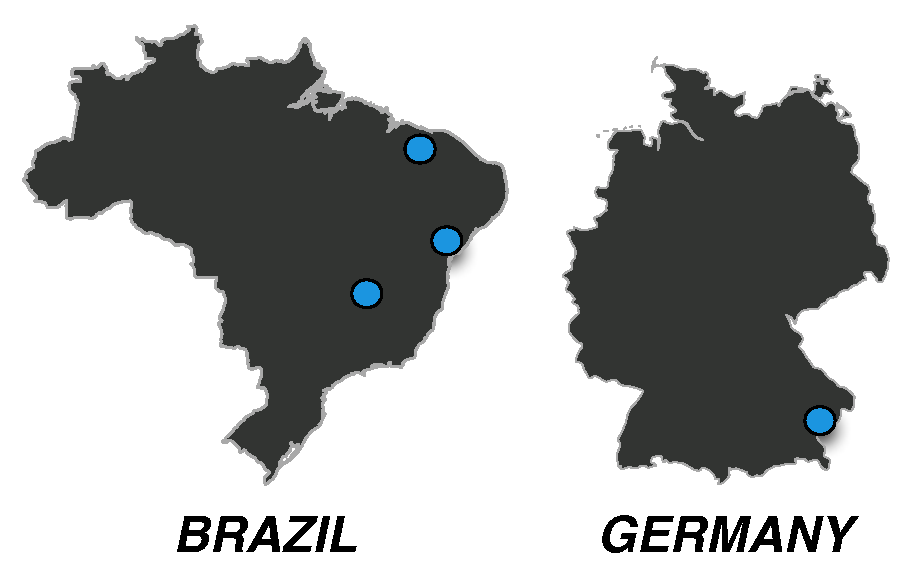
\includegraphics[scale=0.25]{img/places.pdf}
    ~
  \section{Languages}
    \textbf{Portuguese}
\includegraphics[scale=0.40]{img/5stars.png}
    \textbf{English}
\includegraphics[scale=0.40]{img/4stars.png}
    \textbf{German}
\includegraphics[scale=0.40]{img/3stars.png}
    \textbf{Spanish}
\includegraphics[scale=0.40]{img/1stars.png}
    ~
\end{aside}

\section{Publications in Journals}


\includegraphics[scale=0.15]{img/star.pdf}~OLIVEIRA, R. P. ; \textbf{SANTOS, A. R.} ; GOMES, G.; ALMEIDA, E. S..\\
\textbf{Evaluating Lehman's Laws of Software Evolution within Software Product Lines Industrial Projects.}\\
\emph{Journal of Systems and Software . 2016. (In Press)}\\

\textbf{SANTOS, A. R.} ; ALMEIDA, E. S.. \\
\textbf{Do \#ifdef-based Variation Points Realize Feature Model Constraints?}\\
\emph{Software Engineering Notes , v. 40, p. 1-5, 2015.}\\


\section{Publications in Conferences}



\includegraphics[scale=.15]{img/star.pdf}~\textbf{SANTOS, A. R.} ; MACHADO, I. C. ; ALMEIDA, E. S..\\ 
\textbf{RiPLE-HC: JavaScript Systems Meets SPL Composition.}\\
\emph{Proceedings of the 20$^{th}$ Software Product Lines Conference (SPLC). Beijing, 2016. p. 154-163.}\\

\textbf{SANTOS, A. R.}; MACHADO, I. C. ; ALMEIDA, E. S..\\
\textbf{RiPLE-HC: Visual Support for Features Scattering and Interactions.} \\
\emph{Proceedings of the 20$^{th}$ Software Product Lines Conference. Beijing, 2016. p. 320-323.}\\

SOUZA, M. L. J. ; \textbf{SANTOS, A. R.} ; MACHADO, I. C. ; GOMES, G. ; ALMEIDA, E. S..\\
\textbf{Evaluating Variability Modeling Techniques for Dynamic Software Product Lines: A Controlled Experiment.} \\
\emph{Proceedings of the 10$^{th}$ Brazilian Symposium on Components, Architecture, and Reuse (SBCARS). Londrina, 2016. p. 1-10.}\\

 SANTOS, J. A. M. ; \textbf{SANTOS, A. R.}; MENDON\c{C}A, M.. \\
 \textbf{Investigating bias in the search phase of Software Engineering secondary studies.} \\
 \emph{12$^{th}$ Workshop on Experimental Software Engineering. \\
     Proceedings of 18$^{th}$ Ibero-American Conference on Software Engineering (CiBSE), 2015.}\\


\includegraphics[scale=.15]{img/star.pdf}~ \textbf{SANTOS, A. R.}  ; DE OLIVEIRA, R. P.; DE ALMEIDA, E. S..\\
 \textbf{Strategies for consistency checking on software product lines.}\\
 \emph{Proceedings of the 19$^{th}$ International Conference on Evaluation and Assessment in Software Engineering (EASE). Nanjing, 2015.  p. 1-14.}\\
 
SOUZA, M. L. J. ; \textbf{SANTOS, A. R.}  ; ALMEIDA, E. S.. \\
 \textbf{Towards the Selection of Modeling Techniques for Dynamic Software Product Lines.} \\
 \emph{Proceedings of the 5$^{th}$ International Workshop on Product Line Approaches in Software Engineering (PLEASE). Florence, 2015. p. 19-22. }\\
 
\textbf{SANTOS, A. R.}  ; FARIAS, M. A. F. ; ALMEIDA, E. S. ; MENDONCA, M. ; SANTANNA, C. N..\\ 
 \textbf{How developers deal with Code Smells: the case of the SourceMiner Evolution team.} \\
 \emph{Workshop on Software Visualization, Evolution and Maintenance (VEM).
     Proceedings of the 5$^{th}$ Brazilian Conference on Software: Theory and Practice (CBSoft). Maceió, 2014. p. 1-6.}\\
 
VALE, T; CABRAL, B.; ALVIM, L; SOARES, L. ; \textbf{SANTOS, A. R.} ; MACHADO, I.; SOUZA, I.; FREITAS, I.; ALMEIDA, E..\\
  \textbf{SPLICE: A Lightweight Software Product Line Development Process for Small and Medium Size Projects.} \\
 \emph{Proceedings of the 8$^{th}$ Brazilian Symposium on Software Components, Architectures, and Reuse (SBCARS). Maceió, 2014. p. 42-52.}\\
 

\includegraphics[scale=.15]{img/star.pdf}~\textbf{SANTOS, A. R.}  ; GAIA, F. N. ; FIGUEIREDO, E. ; SANTOS NETO, P. ; ARAUJO, J..\\
  \textbf{Test-based SPL extraction: an exploratory study.} \\
  \emph{Proceedings of the ACM Symposium on Applied Computing (SAC). Coimbra, 2013. p. 1031-1036.}\\
  
 SANTOS, I. S. ; \textbf{SANTOS, A. R.}  ; SANTOS NETO, P..\\
 \textbf{Reusing Functional Testing in order to Decrease Performance and Stress Testing Costs.}\\
 \emph{Proceedings of the 23$^{rd}$ International Conference on Software Engineering and Knowledge Engineering (SEKE). Miami, 2011. p. 1-5.}\\
 
    ALVES, P. ; \textbf{SANTOS, A. R.}  ; FIGUEIREDO, E. ; FERRARI, F..\\
    \textbf{How do Programmers Learn AOP? An Exploratory Study of Recurring Mistakes.} \\
    \emph{5$^{th}$ Latin-American Workshop on Aspect-Oriented Software Development (LA-WASP).\\
         Proceedings of the 2$^{nd}$ Brazilian Conference on Software: Theory and Practice (CBSoft). São Paulo, 2011.}\\
    
\section{Honors \& Awards}
\begin{entrylist}
\entry
{2014}
{Best Paper}
{8th International Workshop on Variability Modelling of Software-intensive Systems (VaMoS).}\\
\entry
{2013}
{Travel Award}
{SIGAPP Student Travel Award Program of the Association of Computing Machinery (ACM).}\\
\end{entrylist}

\section{Certifications}
\begin{entrylist}
 \entry
 {2014}
 {English Proficience Level B2}
 {TOEFL ITP}\\
 
 \entry
 {2016}
 {German Proficience Level B2}
 {Volkshochschule Passau}\\
\end{entrylist}

\section{Other Info}
For the Italian job market:\\
\emph{Si autorizza il trattamento delle informazioni contenute nel curriculum in conformità alle disposizioni previste dal d.lgs. 196/2003. Si dichiara altresì di essere consapevole che, in caso di dichiarazioni non veritiere, si è passibili di sanzioni penali ai sensi del DPR 445/00 oltre alla revoca dei benefici eventualmente percepiti.}
\\
\begin{flushleft}
\emph{May 8th, 2016}
\end{flushleft}
\begin{flushright}
\emph{John Snow}
\end{flushright}

\end{document}
